\section{CPU 时间线采样}
这份时间线采于后续 3D 复查之前，保留为测量方法与条件的记录，没有为最终代码重新采集性能结果。
本次在 Windows 11、AMD Ryzen 9 8945HX 上运行一个 256×256 离屏用例。64 个 Opaque 四边形共用网格，深度预传递逐个绘制，主绘制走实例化。预热 10 轮后采集 60 轮，没有场景灯光与 IBL，SSAO 和 RSM 分别使用白色与黑色输入，不执行阴影或后处理。项目 Instrumentor 输出了 300 个同线程事件，原始 JSON 导入 Chrome 157.0.8103.79 的 Performance 面板。

\begin{figure}[H]
\centering
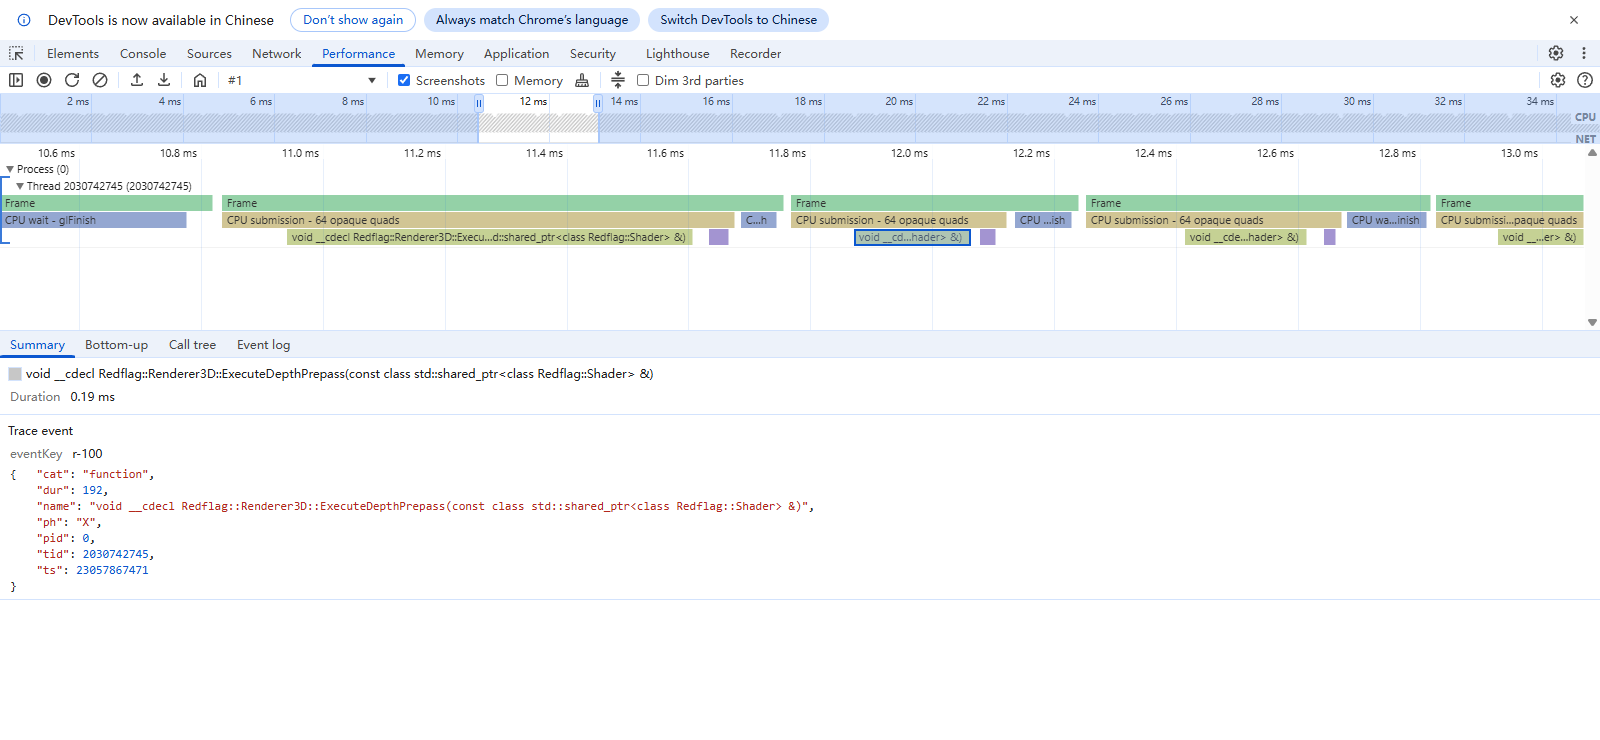
\includegraphics[width=\linewidth]{../../../output/profiling/chrome-cpu-prepass.png}
\caption{Chrome DevTools 实际界面。选中深度预传递的 CPU 区间，原始事件为 192 微秒，界面显示约 0.19 毫秒}
\end{figure}

\begin{tabularx}{\textwidth}{L{6.2cm}Y}
\toprule
CPU 区间 & 60 轮中位数（微秒） \\
\midrule
提交 64 个四边形及两次渲染阶段 & 347 \\
其中：深度预传递 & 199 \\
其中：主绘制 EndScene & 19.5 \\
glFinish 等待 & 66.5 \\
一轮采样 Frame & 467 \\
\bottomrule
\end{tabularx}

这些区间有嵌套关系，不能相加。截图同一轮的 glFinish 等待为 94 微秒，另一张实际截图保存在同目录。它表示 CPU 等待 GPU 完成的时间，不是 GPU 自身执行某个 Pass 的时间。

本次使用 Debug 配置，逐事件写日志并 flush 会干扰采样。每轮 glFinish 又人为串行化了 CPU 与 GPU，没有交换窗口缓冲或完整编辑器工作负载。这里没有优化前后对照，Frame 的倒数不能当作编辑器帧率。后续需要在代表性场景中减少测量干扰并单独获取 GPU 计时。Chrome 的网页专属指标不适用于这份 C++ 时间线。

\note{复现：\path{tests/run_profile_tests.cmd}。原始数据：\path{output/profiling/redflag-cpu-trace.json}，39599 字节；截图和采集说明位于同目录。参考：\source{https://developer.chrome.com/docs/devtools/performance/reference}{Chrome DevTools Performance 功能文档}。}
